% !TEX encoding = UTF-8
% !TEX TS-program = pdflatex
% !TEX root = ../tesi.tex

%**************************************************************
\chapter{Analisi dei requisiti}
\label{cap:analisi dei requisiti}
%**************************************************************

\intro{In questo capitolo viene trattata l'analisi dei requisiti del modulo di front-end della web-app, con i casi d'uso e requisiti fondamentali individuati.}\\

%**************************************************************
\section{Descrizione generale}
\subsection{Interfacce della web-app}
\subsubsection{Interfaccia menù}
L'utente può visualizzare il menù del ristorante dopo aver scansionato il QR-code presente sui tavoli. Il menù è composto da un insieme di categorie, in ognuna di esse sono presenti dei piatti. I piatti sono ordinati in base al loro id, che è un numero univoco dentro ogni menù.
\subsubsection{Interfaccia lista degli ordini}
L'utente può vedere i piatti ordinati del suo tavolo, dove ci sono anche i piatti ordinati dalle altre persone dello stesso tavolo, inoltre può vedere i suoi piatti personali e i piatti in arrivo.
\subsubsection{Interfaccia gestione del tavolo}
In questa \gls{mascherag} un utente può creare la \gls{sessioneg} del tavolo se non è stata già creata, altrimenti può visualizzare il QR-code della sua sessione per permettere ad altri utenti di partecipare.
\subsubsection{Interfaccia area personale}
Qui l'utente può effettuare il login e successivamente se ha delle allergie potrà inserire degli ingredienti nella blacklist per nascondere i piatti dal menù che contengono quest'ultimi.
\subsection{Caratteristiche degli utenti}
In questa sezione vengono descritti tutte le caratteristiche degli utenti che possono utilizzare la web-app.
\subsubsection{Utente non autenticato}
Con il termine utente non autenticato ci si riferisce ad una qualsiasi persona non autenticata nel sistema, che può sfruttare le funzionalità di base offerte dalla piattaforma, ossia:
\begin{itemize}
    \item Visualizzare il menù del ristorante;
    \item Visualizzare i singoli piatti in modalità dettaglio;
    \item Creare una sessione di un tavolo;
    \item Partecipare ad una sessione già esistente di un tavolo;
    \item Uscire dalla sessione di un tavolo;
    \item Aggiungere piatti negli ordini;
    \item Aggiungere note ai piatti ordinati;
    \item Spostare ordini in arrivo;
    \item Marcare un piatto in arrivo come arrivato;
    \item Effettuare la registrazione nella piattaforma;
    \item Effettuare il login.
\end{itemize}
\subsubsection{Utente autenticato}
Invece, con il termine “utente autenticato” ci si riferisce ad una persona registrata nel database e che ha effettuato l'accesso nella piattaforma, la quale, oltre a sfruttare le funzionalità dell'utente non autenticato, può anche:
\begin{itemize}
    \item Aggiungere piatti nei preferiti;
    \item Rimuovere piatti dai preferiti;
    \item Dare una recensione ad un piatto;
    \item Aggiungere ingredienti alla blacklist;
    \item Rimuovere gli ingredienti dalla blacklist;
    \item Visualizzare la lista dei preferiti;
    \item Effettuare il logout.
\end{itemize}
%**************************************************************
\subsection{Tecnologie utilizzate}
Per sviluppare la piattaforma vengono utilizzate le seguenti tecnologie:
\begin{itemize}
    \item Angular: per la creazione dell'interfaccia utente;
    \item HTML5: per creare la struttura dell'interfaccia utente;
    \item CSS3: per lo stile dell'interfaccia, viene utilizzata la sintassi SCSS;
    \item Stoplight: per simulare le chiamate REST \gls{apig};
    \item Angular Material: per la creazione dei componenti.
\end{itemize}
\subsection{Descrizione delle tecnologie}
\subsubsection{Angular}
Angular è un framework open source per sviluppare applicazioni web, permette di dividere l'applicazione in più componenti, grazie a questo è possibile riutilizzare lo stesso modulo in più parti della web-app ed inoltre garantisce una maggiore manutenibilità e espandibilità.
\begin{figure}[H]
    \centering
    
\includegraphics[scale=0.1]{angular.png}
    \caption{Logo di Angular}
\end{figure}
\subsubsection{HTML5}
L'HyperText Markup Language, noto come HTML, è il linguaggio di markup più popolare, utilizzato per progettare le strutture dei siti web. Viene utilizzato da Angular per creare la struttura iniziale delle varie interfacce che verranno a seguito modificate da Angular per generare la pagina dinamicamente.
\begin{figure}[H]
    \centering
    
\includegraphics[scale=0.5]{html css.png}
    \caption{Logo di HTML e CSS}
\end{figure}
\subsubsection{CSS3}
Il CSS, sigla di Cascading Style Sheets, è il linguaggio utilizzato per modificare il layout delle pagine web, le regole vengono applicate nell'ordine in cui vengono scritte. Per il progetto è stata utilizzata una sua estensione SCSS, la quale è compatibile con tutte le versioni di CSS. Tramite SCSS è possibile dichiarare le regole CSS in blocchi il che aiuta a scrivere regole CSS in modo più veloce e comprensibile.
\subsubsection{TypeScript}
% Il linguaggio di programmazione utilizzato da Angular è TypeScript, un linguaggio di programmazione open source sviluppato da Microsoft,
TypeScript è un linguaggio di programmazione open source sviluppato da Microsoft ed utilizzato da Angular, il quale estende il classico JavaScript perciò è in grado di eseguire qualsiasi programma scritto in JavaScript senza nessuna modifica. TypeScript rende molto più flessibile JavaScript aggiungendo la firma dei metodi, classi, tipi di dato e tanto altro, questo permette di effettuare controlli automatici e rilevare i bug in fase di compilazione. Grazie a TypeScript il codice generato da Angular è eseguibile su tutti i pricipali web browser come Google Chrome, Firefox, Safari, Opera, Microsoft Edge e tanti altri.
\subsubsection{Stoplight}
Stoplight è una piattaforma che offre la possibilità di realizzare le API, grazie alla sua semplice interfaccia utente ne velocizza la progettazione. Permette di collaborare con gli altri, condividendo tutte le API e mostrando per ognuna di esse l'endpoint, la descrizione e la risposta.
\begin{figure}[H]
    \centering
    
\includegraphics[scale=0.4]{stoplight logo.png}
    \caption{Logo di Stoplight}
\end{figure}
\subsubsection{Angular Material}
Angular Material è un insieme di componenti grafici web già implementati, questi componenti possono essere direttamente utilizzati in Angular. Tutti i componenti offerti sono \gls{responsiveg} e liberamente modificabili.
\begin{figure}[H]
    \centering
    
\includegraphics[scale=0.3]{angular material.png}
    \caption{Logo di Angular Material}
\end{figure}
\section{Casi d'uso}
\subsection{Introduzione}
In questa sezione verranno presentati i casi d'uso individuati durante la fase di analisi dei requisiti, i quali fanno riferimento a tutte le funzionalità che la web-app SushiLab dovrà offrire ad ogni utente che vorrà interfacciarsi con essa. Verranno elencati i casi d'uso principali con la propria descrizione, mentre i casi d'uso secondari e le descrizioni schematiche potranno essere reperiti nell'appendice {\hyperref[cap:appendice a]{A}}.
\subsection{Attori primari}
\begin{itemize}
    \item Utente non Autenticato: utente che non ha ancora effettuato l'autenticazione sulla piattaforma. Può essere in possesso o meno delle credenziali per l'autenticazione. Ha funzionalità limitate rispetto ad un utente autenticato;
    \item Utente Autenticato: utente che ha effettuato l'autenticazione alla piattaforma tramite le proprie credenziali. Ha accesso ad ogni funzionalità messa a disposizione dalla piattaforma;
    \item  Utente Generico: può essere sia un utente autenticato che un utente non autenticato.
\end{itemize}
\subsubsection{UC1 - Visualizza menù}
La schermata di visualizzazione menù consente di effettuare operazioni relative all'acquisto dei piatti in base alla tipologia di utente che interagisce con la piattaforma.
Un utente generico può visualizzare un piatto in due modalità quella normale e quella in dettaglio.\\
In quella normale vengono visualizzati il nome, la descrizione, gli ingredienti e il prezzo, ed è possibile modificare la quantità dei piatti ordinati.
Nella modalità in dettaglio l'utente può visualizzare la valutazione media e, opzionalmente, può aggiungere una nota al piatto.\\
L'autenticazione dell'utente nel sistema permette svolgere ulteriori azioni, quali:\\
\begin{itemize}
    \item L'aggiunta di un piatto alla lista dei preferiti per tenere traccia dei migliori piatti ordinati;
    \item La visualizzazione del menù calibrato sulla blacklist dell'utente;
    \item Recensire pubblicamente un piatto del menù con una valutazione da una a cinque stelle.
\end{itemize}
% \begin{figure}[H]
%     \centering
%     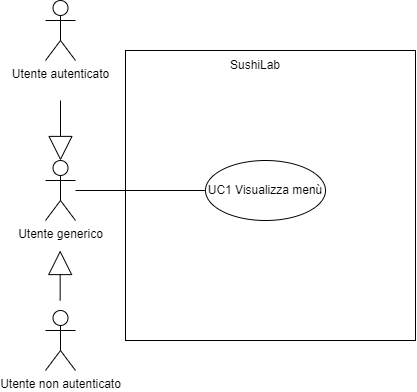
\includegraphics[scale=0.5]{usecase/tesi-uc1.drawio.png}
%     \caption{Use Case - UC 1}
% \end{figure}
% \begin{figure}[H]
%     \centering
%     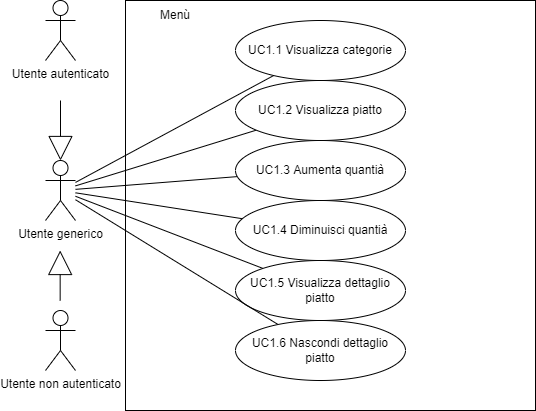
\includegraphics[scale=0.5]{usecase/tesi-uc11.drawio.png}
%     \caption{Use Case - UC 1.1, UC 1.2, UC 1.3, UC 1.4, UC 1.5, UC 1.6}
% \end{figure}
\subsubsection{UC2 - Gestione del tavolo}
La schermata di gestione del tavolo consente di effettuare operazioni relative alla sessione del tavolo. Scansionando il QR-code l'utente visualizza la pagina per la gestione del tavolo che permette di creare la sessione all'interno della web-app o di partecipare a quella già esistente. Dopo aver creato la sessione l'utente può generare il relativo QR-code o un codice alfanumerico per permettere ad altre persone di unirsi. In ogni momento un utente può abbandonare la sessione in cui partecipa.
% \begin{figure}[H]
    % \centering
    % 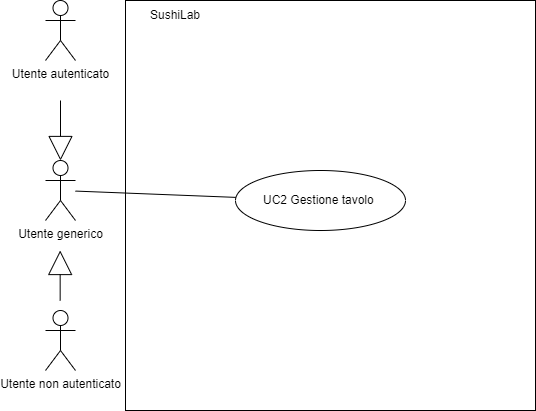
\includegraphics[scale=0.5]{usecase/tesi-uc2.drawio.png}
    % \caption{Use Case - UC 2}
% \end{figure}
% \begin{figure}[H]
    % \centering
    % 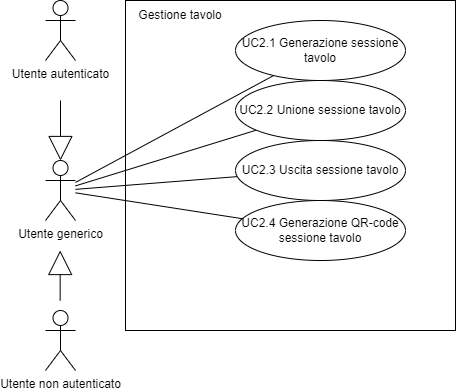
\includegraphics[scale=0.5]{usecase/tesi-uc21.drawio.png}
    % \caption{Use Case - UC 2.1, UC 2.2, UC 2.3, UC 2.4}
% \end{figure}
\subsubsection{UC3 - Lista degli ordini}
La maschera della lista degli ordini si compone di tre sezioni, quali: \gls{ordinitavolog}, \gls{ordiniinarrivog} e \gls{ordinipersonalig}.
La sezione degli ordini del tavolo permette di visualizzare gli ordini di tutti gli utenti partecipanti alla stessa sessione, questi rappresentano gli ordini non ancora inviati al ristorante e possono quindi essere modificati. L'utente può generare tramite l'app il QR-code degli ordini da scannerizzare per inviare l'ordine alla cucina.
La lista degli ordini in arrivo permette di visualizzare i piatti in preparazione.
Infine la sezione degli ordini personali contiene lo storico dei piatti ordinati durante la sessione in cui si trova l'utente, permettendogli di visualizzare tutte le caratteristiche di un piatto, la nota e la quantità ordinata.
% \begin{figure}[H]
%     \centering
%     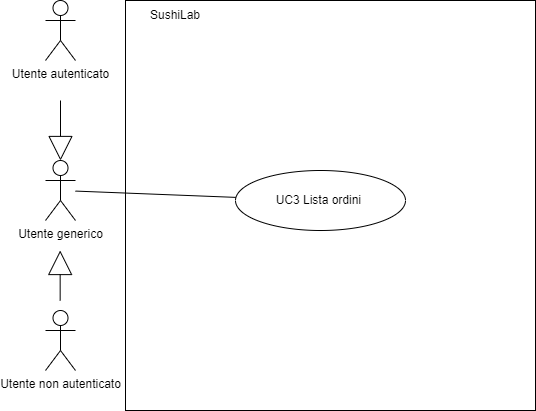
\includegraphics[scale=0.5]{usecase/tesi-uc3.drawio.png}
%     \caption{Use Case - UC 3}
% \end{figure}
% \begin{figure}[H]
%     \centering
%     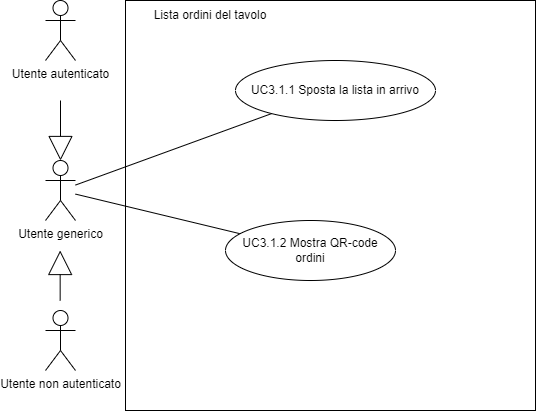
\includegraphics[scale=0.5]{usecase/tesi-uc311.drawio.png}
%     \caption{Use Case - UC 3.1, UC 3.2, UC 3.3}
% \end{figure}
% \begin{figure}[H]
%     \centering
%     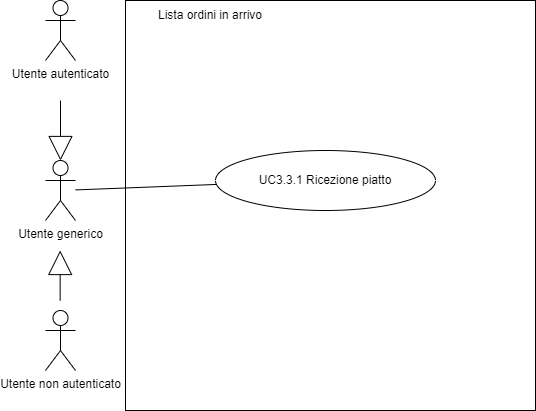
\includegraphics[scale=0.5]{usecase/tesi-uc333.drawio.png}
%     \caption{Use Case - UC 3.3.1}
% \end{figure}
\subsubsection{UC4 - Area personale}
La pagina dell'area personale permette all'utente non autenticato di effettuare il login nella piattaforma tramite l'email e la password per accedere alle funzionalità complete dell'applicazione, di registrarsi su sushiLab e di effettuare il recupero delle credenziali. In seguito all'autenticazione l'utente può accedere e modificare la propria blacklist degli ingredienti.
\section{Requisiti}
In base a quanto definito nell'analisi dei requisiti è stata individuata una lista di requisiti che deve essere soddisfatta al termine del progetto di stage. Per ogni requisito individuato è stato assegnato un codice univoco, la descrizione del requisito e il caso d'uso riferito. Tutti i requisiti sono mostrati dentro una tabella e può essere reperita nell'appendice {\hyperref[cap:appendice b]{B}}.
\subsection{Panoramica}
Un utente che accede al sistema deve potersi autenticare e registrare fornendo un'email e una password.
L'utente deve poter accedere alla sezione del menù visualizzando tutti i piatti oppure quelli filtrati. I piatti del menù si possono visualizzare in modalità normale e dettagliata ed essere aggiunti agli ordini. L'utente deve essere in grado di creare, partecipare o uscire da una sessione di un tavolo. All'interno di una sessione l'utente deve poter visualizzare le liste degli ordini del tavolo, in arrivo e quelli personali mostrando per ogni ordine il nome, la descrizione e l'immagine dei piatti contenuti. Per ogni ordine del tavolo l'utente deve poter generare un codice-QR per l'invio di quest'ultimo. I piatti inviati vengono poi spostati nella lista degli ordini in arrivo. Un utente autenticato deve essere in grado di recensire un piatto, aggiungerlo alla propria lista dei preferiti e modificare la propria blacklist degli ingredienti. Infine in caso di smarrimento della password l'utente deve poter effettuare la richiesta di recupero fornendo l'email.